\documentclass{standalone}
\usepackage{tikz}

\begin{document}
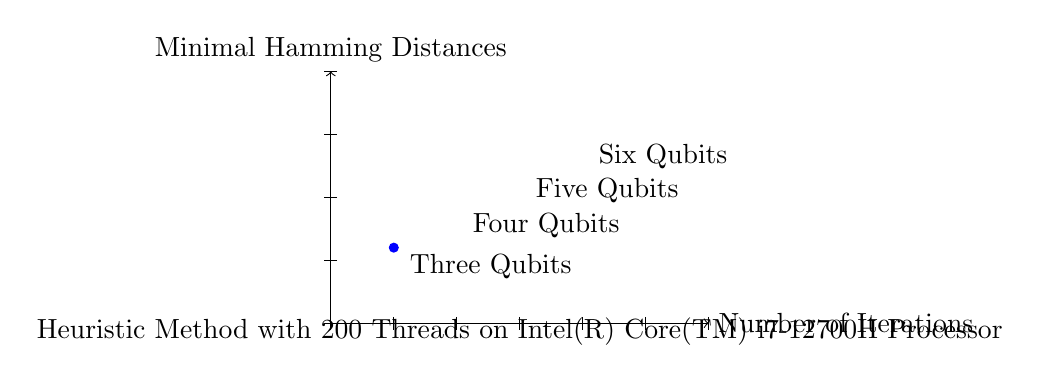
\begin{tikzpicture}[scale=0.8]
    % Define colors
    \definecolor{blue}{RGB}{0,0,255}
    \definecolor{green}{RGB}{0,255,0}
    \definecolor{red}{RGB}{255,0,0}

    % Axes
    \draw[->] (0,0) -- (6,0) node[right] {Number of Iterations};
    \draw[->] (0,0) -- (0,4) node[above] {Minimal Hamming Distances};

    % Data points
    \filldraw[blue] (1,1.2) circle[radius=2pt];
    \filldraw[green] (2,1.8);
    \filldraw[red] (3,2.4);

    % Labels for data points
    \node at (1.1,1.25) [below right] {Three Qubits};
    \node at (2.1,1.9) [below right] {Four Qubits};
    \node at (3.1,2.45) [below right] {Five Qubits};
    \node at (4.1,3.0) [below right] {Six Qubits};

    % Plot title
    \node at (3,-0.5) [above] {Heuristic Method with 200 Threads on Intel(R) Core(TM) i7-12700H Processor};

    % Grid
    \foreach \x in {0,1,...,6} \draw (\x,0.1) -- (\x,-0.1);
    \foreach \y in {0,1,...,4} \draw (0.1,\y) -- (-0.1,\y);
\end{tikzpicture}
\end{document}